\section{Ergebnisse}
\label{sec:ergebnisse}

Als Basis f\"ur eine Ergebnisdiskussion sind in
Abbildung~\ref{fig:modellvorhersagen} die vorhergesagten Nummernschilder
f\"ur 10 Testbilder zu sehen, die alle weder beim Training noch bei der
Validierung zum early stopping verwendet wurden.

Was den ersten Teil der Pipeline angeht, also die Bildsegmentierung
mithilfe eines CNN, so l\"asst sich erkennen, dass das CNN f\"ur jedes
der Bilder den relevanten Bereich, der das Nummernschild enth\"alt,
korrekt vorhersagen konnte.
Selbst die sehr abgedunkelten Lichtverh\"altnisse in Bild (i) konnten
die Vorhersage nicht negativ beeintr\"achtigen.
Dies kann als Anzeichen gedeutet werden, dass es sich hier um eine
sehr vielversprechende Technologie handeln k\"onnte, was das Auffinden
der Nummernschilder angeht.
Die Vorhersagen k\"onnen also als proof-of-concept f\"ur den ersten
Teil der Pipeline dienen.

Was den zweiten Teil der Pipeline, also die Texterkennung angeht, so
fallen leider teils eklatante M\"angel ins Auge.
Lediglich bei einem einzigen Bild (Bild (a)) wurde das Nummernschild
korrekt ausgelesen. Ansonsten sind die Vorhersagen von vielen
Schwachstellen gepr\"agt.
Ein Fehler, der h\"aufig vorkommt, ist das scheinbar
willk\"urliche Verdoppeln gelesener Zeichen, wie es beispielsweise
in Bild (h) und auch in Bild (j) zu sehen ist.
Dar\"uber hinaus passiert es wie in Bild (d) und (g) h\"aufig, dass
einige Zeichen garnicht erst erkannt werden.
In Bild (f) wurde sogar, obwohl der Bereich des Nummernschildes zuvor
richtig ausgelesen wurde, kein einziges Zeichen erkannt.

Es l\"asst sich insgesamt also erkennen, dass die Texterkennung
der aktuelle Problempunkt in der Pipeline ist.
Im folgenden sind ein paar Ideen aufgef\"uhrt, wie dieser Teil
der Pipeline in Zukunft verbessert werden k\"onnte.

\subsection{Ideen zur Verbesserung der Texterkennung}

\paragraph{Framework zur iterativen Verbesserung}

Bevor konkrete Verbesserungsans\"atze eingebracht werden k\"onnen bedarf
es zun\"achst eines Frameworks, also einer allgemeinen Vorgehensweise,
wie zielgerichtet gearbeitet werden kann, um die Pipeline zu verbessern.
Ein m\"oglicher Ansatz ist es, sich zuerst auf eine Metrik festzulegen,
die die Qualit\"at
der Pipeline beschreibt und dann anhand dieser Metrik m\"ogliche
\"Anderungen und Verbesserungen zu beurteilen.
Neuerungen w\"urden nur dann akzeptiert werden, wenn sie auch zu einer
Verbesserung der zu Anfang festgelegten Metrik f\"uhren.

Eine m\"ogliche Metrik, die in diesem Kontext sinnvoll erscheint,
ist die Levenshtein-Distanz, die erstmals in~\cite{levenshtein}
eingef\"uhrt wurde.
Die Levenshtein-Distanz gibt an, wieviele Einf\"uge-, L\"osch- und
Ersetz-Operationen notwendig sind, um eine Zeichenkette in eine
andere zu \"uberf\"uhren.
In der hier vorliegenden Situation k\"onnte man also die
Levenshtein-Distanzen zwischen den Modellvorhersagen und den
tats\"achlichen Nummernschildern messen und so eine Aussage \"uber
die Qualit\"at der Pipeline erhalten.

Zur Verbesserung der Texterkennung k\"onnte man nun also einen Teil der
Daten beiseite legen, beispielsweise die Bilder in Abbildung~\ref{fig:modellvorhersagen},
und sich als Ziel setzen, die mittlere Levenshtein-Distanz der
Pipeline auf diesen Bildern zu minimieren.
Hierbei k\"onnte man dann iterativ vorgehen: Hat man eine Idee zur
Verbesserung der Pipeline entwickelt, so wird diese anhand der
mittleren Levenshtein-Distanz auf den Testdaten evaluiert.
Nur dann, wenn die mittlere Levenshtein-Distanz durch das Einbringen
dieser Idee verkleinert werden konnte, wird die Idee in die Pipeline
aufgenommen.

\paragraph{Einfache Testf\"alle als \glqq Sanity Checks\grqq{}}

\paragraph{Wechsel der Technologie}

\begin{figure}
    \centering
    \begin{subfigure}{0.31\textwidth}
        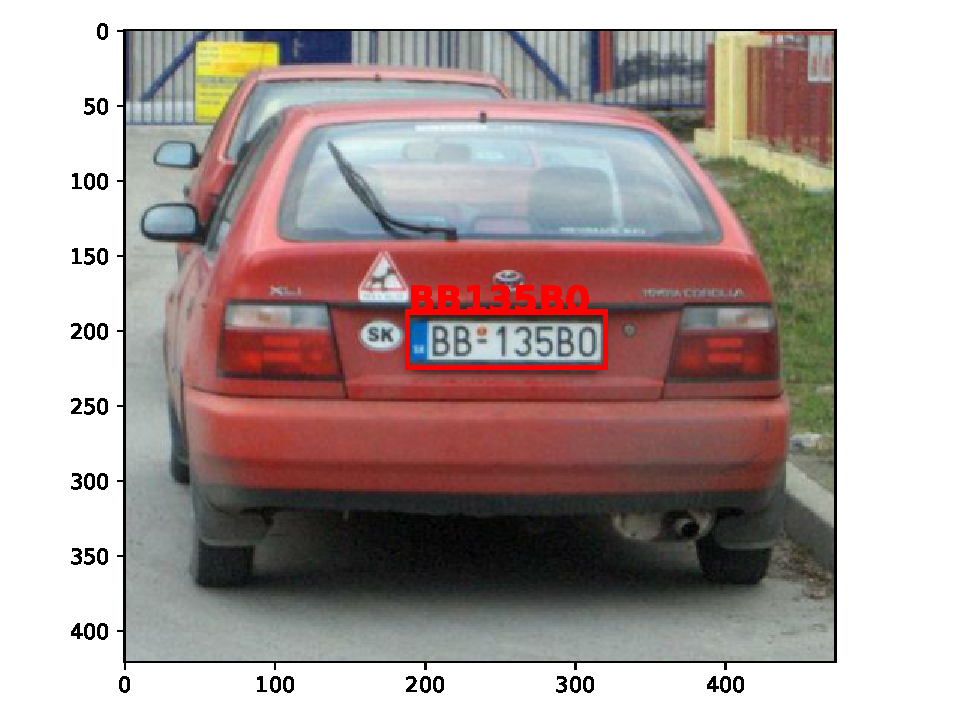
\includegraphics[width=\textwidth]{abbildungen/prediction_01.pdf}
        \subcaption{Vorhersage: BB135B0}
    \end{subfigure}
    \begin{subfigure}{0.31\textwidth}
        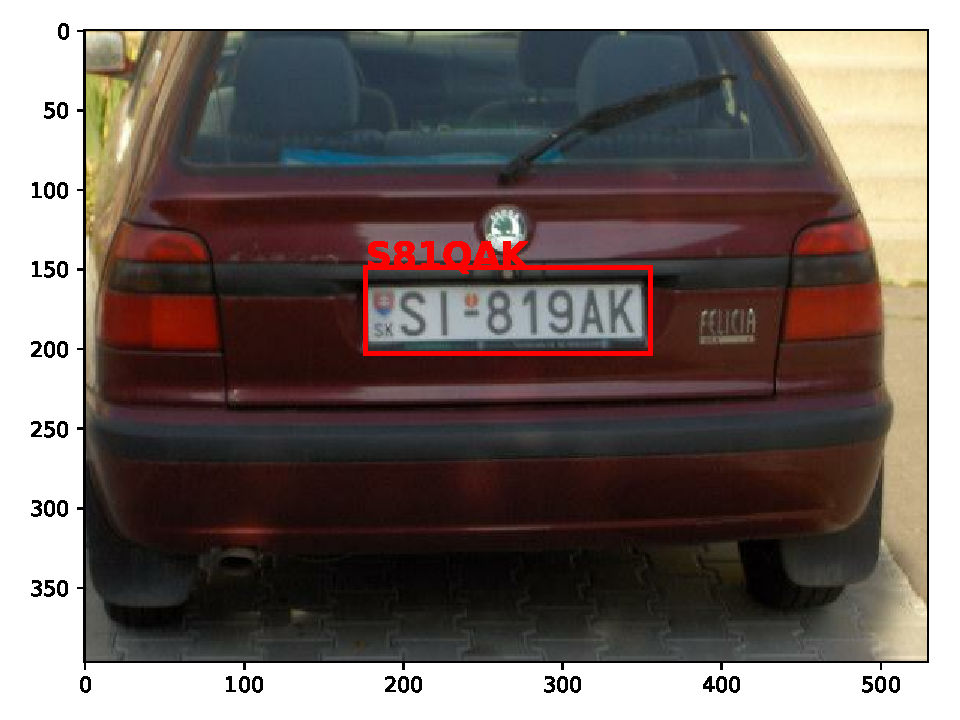
\includegraphics[width=\textwidth]{abbildungen/prediction_02.pdf}
        \subcaption{Vorhersage: S81QAK}
    \end{subfigure}
    \begin{subfigure}{0.31\textwidth}
        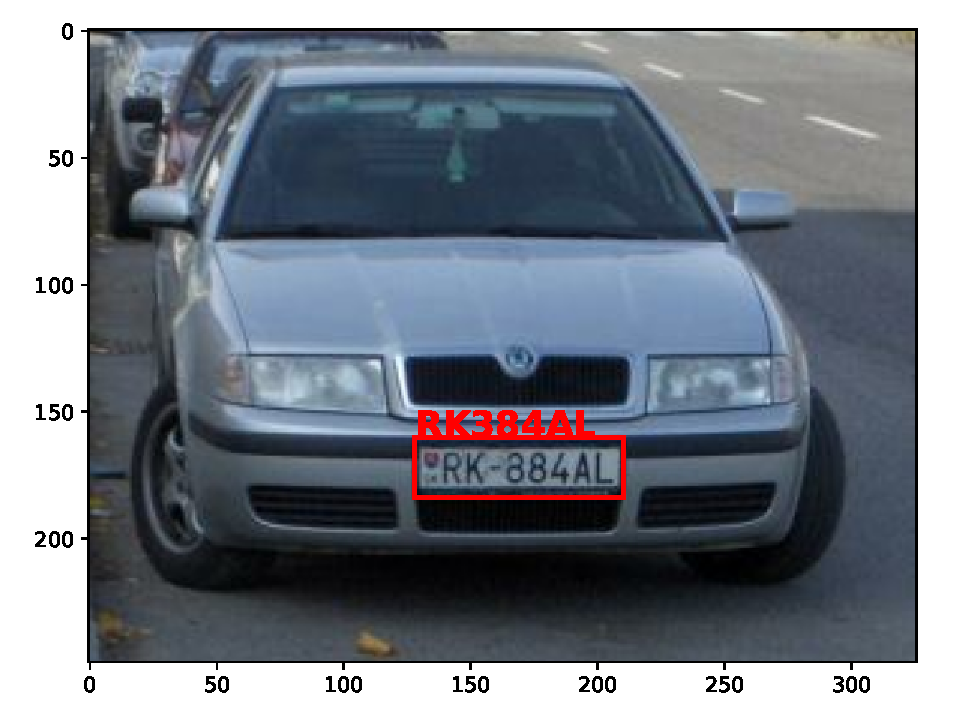
\includegraphics[width=\textwidth]{abbildungen/prediction_03.pdf}
        \subcaption{Vorhersage: RK384AL}
    \end{subfigure}
    \begin{subfigure}{0.31\textwidth}
        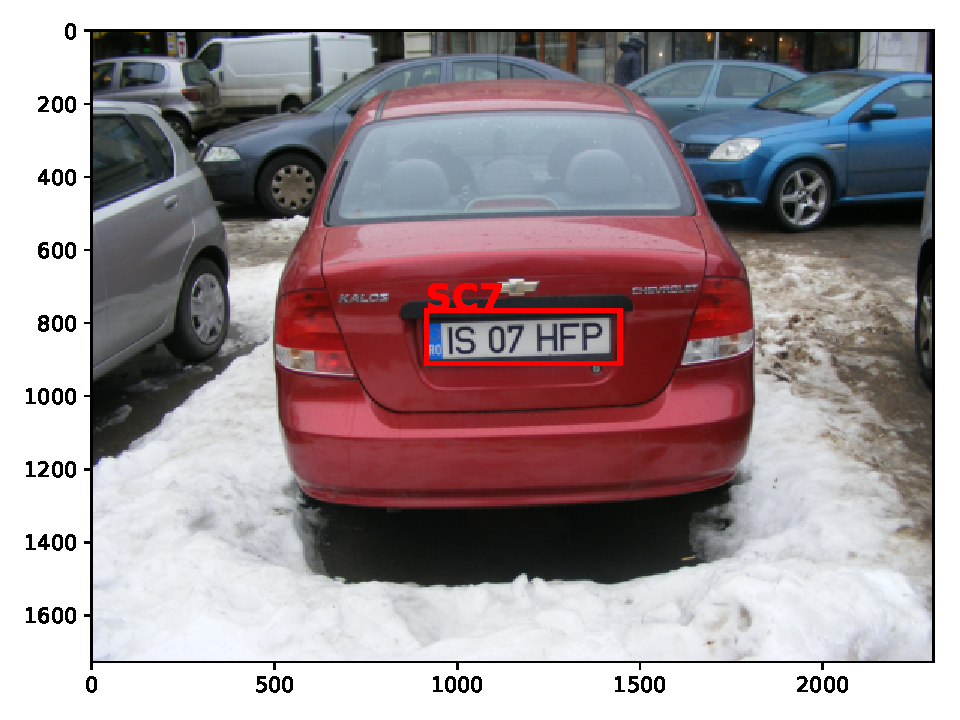
\includegraphics[width=\textwidth]{abbildungen/prediction_04.pdf}
        \subcaption{Vorhersage: SC7}
    \end{subfigure}
    \begin{subfigure}{0.31\textwidth}
        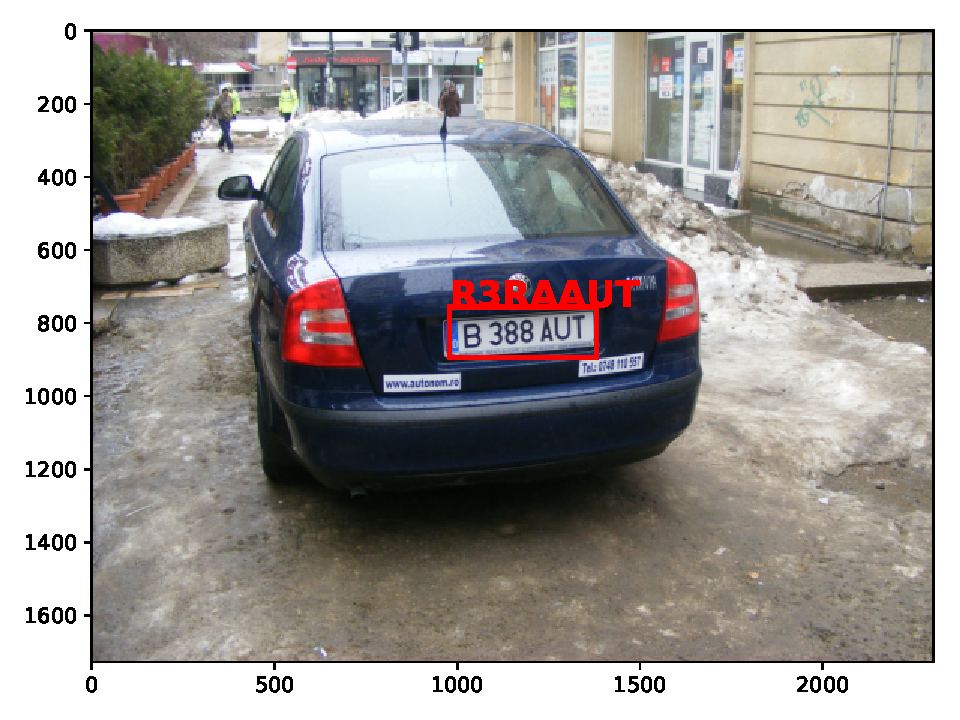
\includegraphics[width=\textwidth]{abbildungen/prediction_05.pdf}
        \subcaption{Vorhersage: R3RAAUT}
    \end{subfigure}
    \begin{subfigure}{0.31\textwidth}
        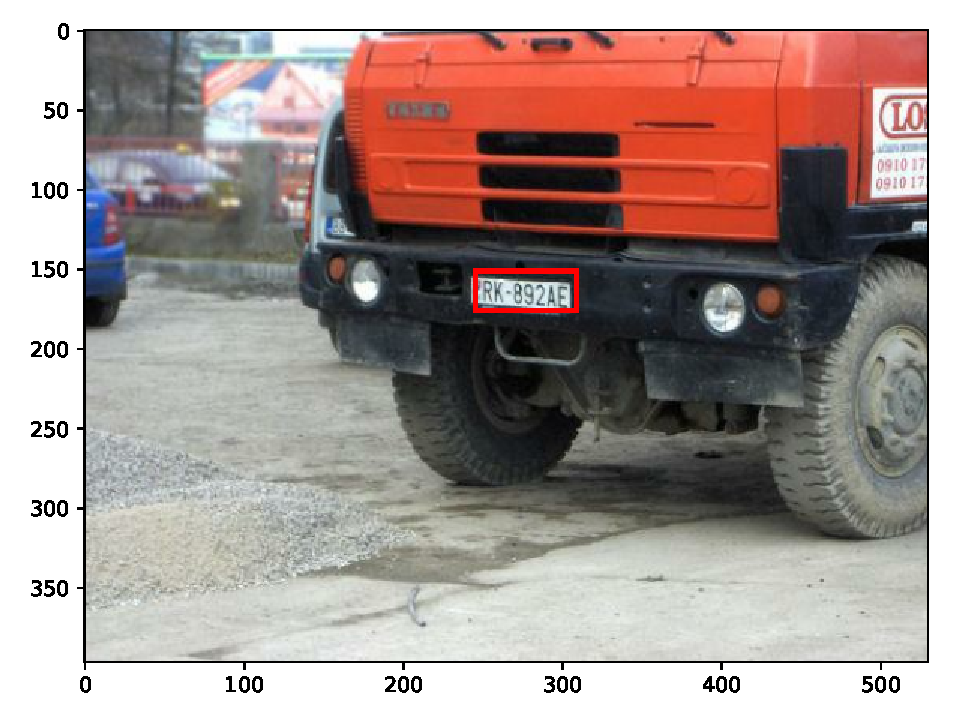
\includegraphics[width=\textwidth]{abbildungen/prediction_06.pdf}
        \subcaption{Vorhersage: -}
    \end{subfigure}
    \begin{subfigure}{0.31\textwidth}
        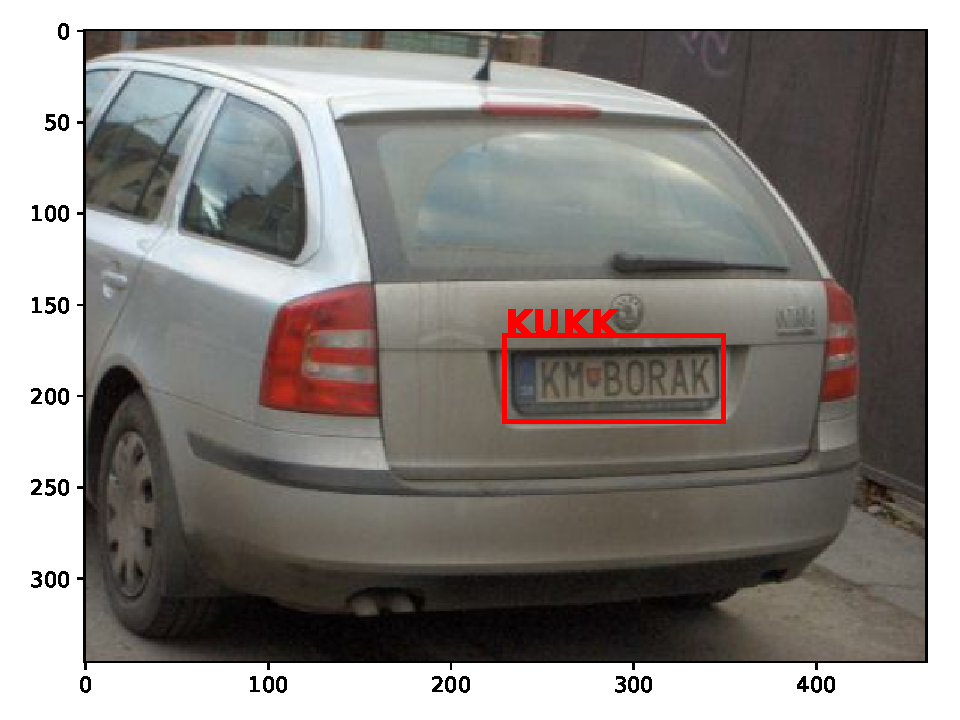
\includegraphics[width=\textwidth]{abbildungen/prediction_07.pdf}
        \subcaption{Vorhersage: KUKK}
    \end{subfigure}
    \begin{subfigure}{0.31\textwidth}
        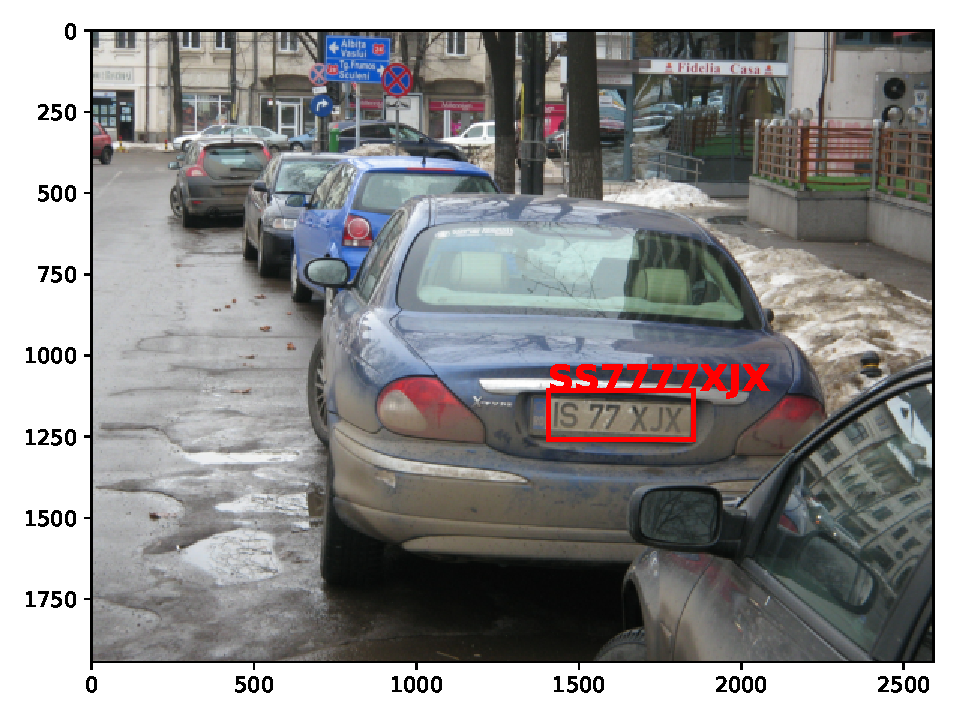
\includegraphics[width=\textwidth]{abbildungen/prediction_08.pdf}
        \subcaption{Vorhersage: SS7777XJX}
    \end{subfigure}

    \begin{subfigure}{0.31\textwidth}
        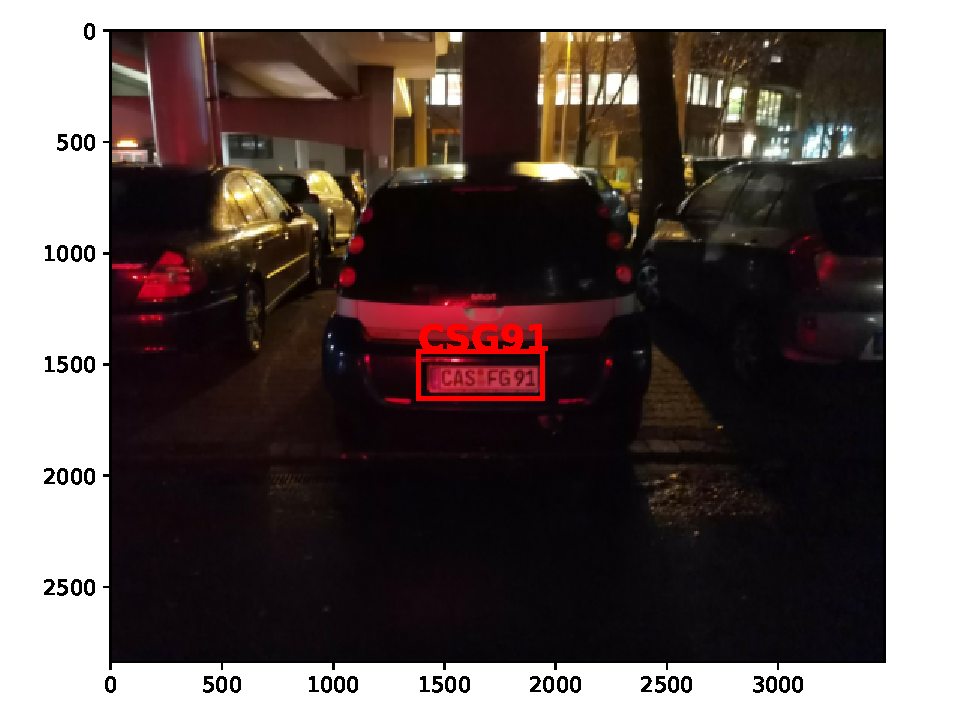
\includegraphics[width=\textwidth]{abbildungen/prediction_09.pdf}
        \subcaption{Vorhersage: CSG91}
    \end{subfigure}
    \begin{subfigure}{0.31\textwidth}
        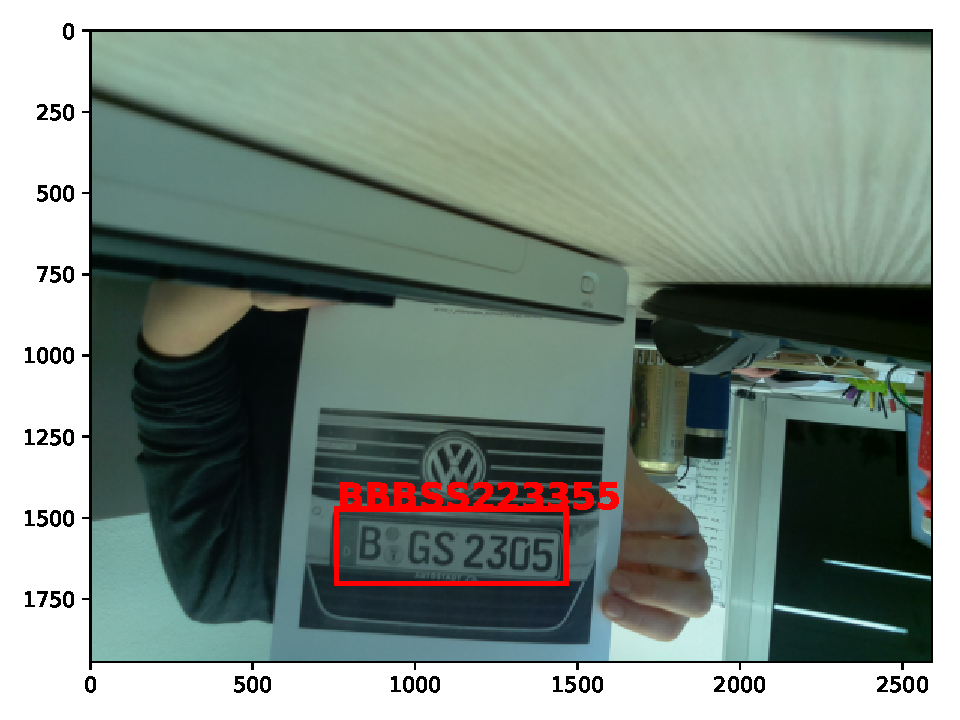
\includegraphics[width=\textwidth]{abbildungen/prediction_10.pdf}
        \subcaption{Vorhersage: BBBSS223355}
    \end{subfigure}
    \caption[Modellvorhersagen]{Modellvorhersagen f\"ur 10 ungesehene Testbilder.
        Die vorhergesagten Nummernschilder sind durch rote Rechtecke markiert.}
    \label{fig:modellvorhersagen}
\end{figure}
